\subsection{Static Perfomance}

\subsubsection{Excess Thrust}

In fig.~\ref{fig:Tex_Graph} the Excess Thrust with regards to the Mach number is presented:

\begin{figure}[H]
    \centering
    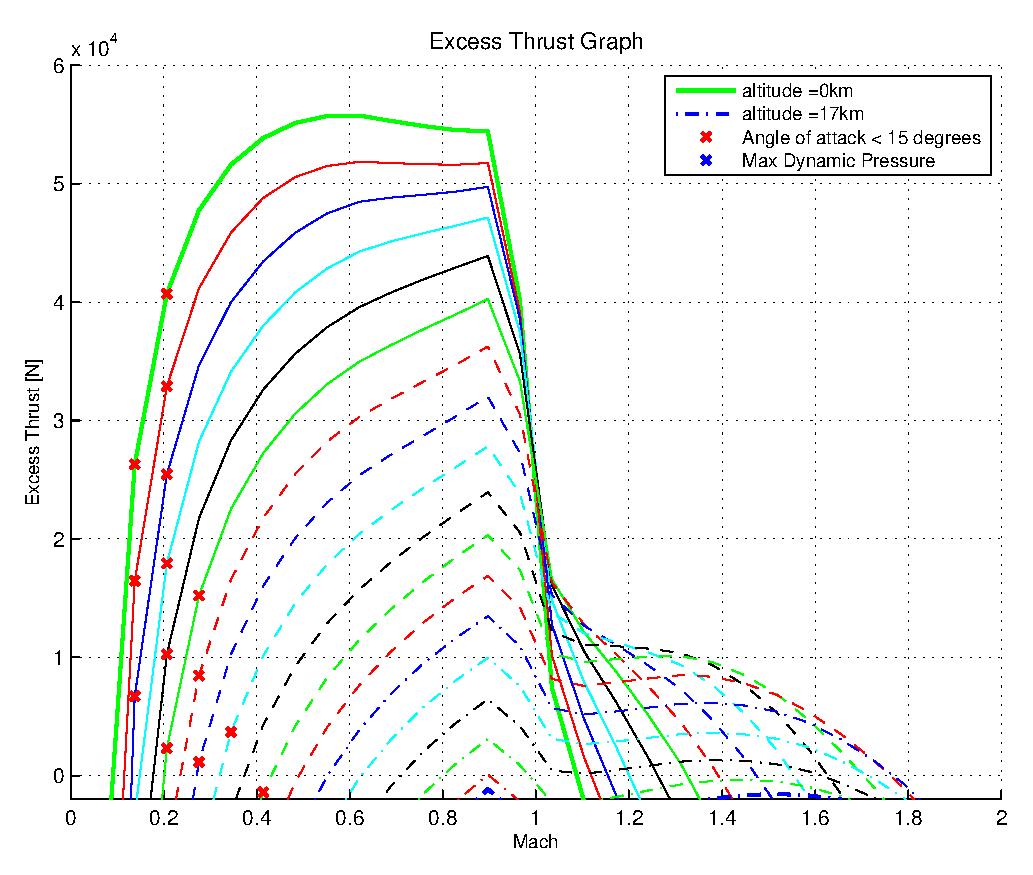
\includegraphics[width=1.0\textwidth]{Tex_Graph}
    \caption{Excess Thrust Graph}
    \label{fig:Tex_Graph}
\end{figure}

Using the graph we can now determine the envelope limits corresponding to the dynamic pressure and the 
maximum angle of attack. These limits are shown in the diagram as red and blue Xs.
We should note however that the dynamic pressure limits are not visible in  \ref{fig:Tex_Graph}, when presenting 
only the part of the diagram above the zero horizontal line.

\subsubsection{SEP Graph}

\noindent Having computed the Excess thrust of the aircraft model, we can now 
compute the Specific Excess Power and then form the Envelope graph of the Draken J35 by using
eq.~\ref{eqn:SEP}. The envelope graph is presented in fig.~\ref{fig:SEP_Graph}.

\begin{figure}[H]
    \centering
    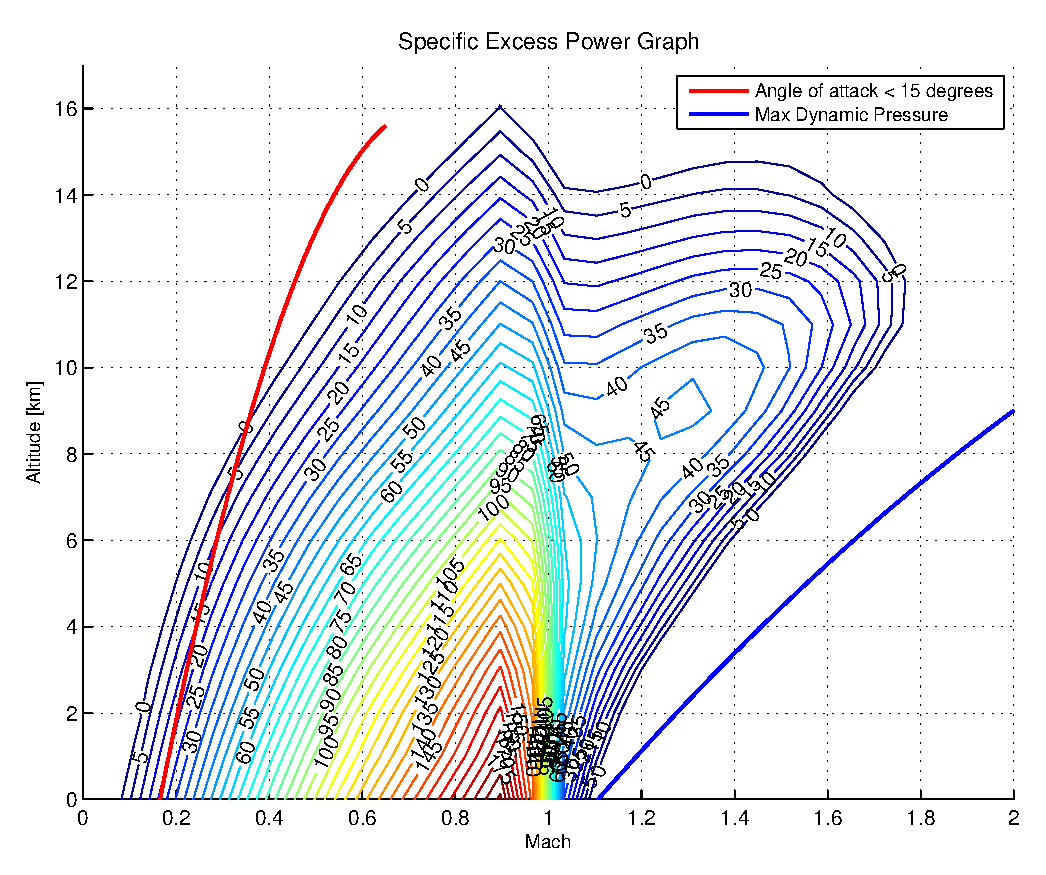
\includegraphics[width=1.0\textwidth]{SEP_Graph}
    \caption{SEP Graph}
    \label{fig:SEP_Graph}
\end{figure}

\noindent Graph \ref{fig:SEP_Graph} shows the contours of same Excess Power with regards to
the altitude of the airplane as well as the Mach number thus the velocity of the airplane.

Using this graph we can also determine the envelope limits corresponding to the maximum angle of attack
$(15^{\degree})$ and the maximum dynamic pressure corresponding to $1350 \sfrac{km}{h}$ at sea level which 
is $8.6133e^{+04}\, Pa$.

\subsection{Maximum altitude - Maximum Mach Number}
The maximum altitude and the maximum Mach Number at which the aircraft can fly level 
can be determined using \ref{fig:SEP_Graph}:

\begin{itemize*}
    \item Max. Altitude: 16 km
    \item Max Mach: 1.76
\end{itemize*}
